\documentclass[12pt]{article}
\usepackage[utf8]{inputenc}
\usepackage[spanish]{babel}
\usepackage{graphicx}
\usepackage{float}
\usepackage{caption}
\usepackage{csquotes}
\usepackage{booktabs}
\usepackage{amsmath}
\usepackage{hyperref}
\usepackage[backend=biber,style=apa]{biblatex}
\addbibresource{../../referencias/referencias.bib}
\usepackage{geometry}
\usepackage{url}
\geometry{margin=2.5cm}



\begin{document}
\begin{titlepage}
\centering
\vspace*{\fill}

{\Huge\bfseries Bitácora 4\par}
\vspace{1.5cm}

{\Large\textbf{Integrantes:}\par}
Debbie Con Ortega (C32250)\\
Ashly Garro Villanueva (C33198)\\
Emily Sanchéz Mancía (C27260)\\
Alessandro Umaña Vega (C37963)

\vspace{1cm}

{\Large\textbf{Profesor:} Maikol Solís\par}
\vspace{1.5cm}

{\Large I Ciclo 2026\par}

\vspace*{\fill}
\end{titlepage}
\tableofcontents
\newpage
\section{Parte de escritura}
\subsection{Escritura}
El análisis de la siniestralidad vial constituye uno de los desafíos más críticos 
para la salud pública a nivel global. Comprender las interacciones de factores que 
desencadenan un siniestro resulta fundamental para el diseño de políticas públicas 
eficaces. Esta investigación busca resolver qué combinaciones de factores del entorno 
ocurren con mayor frecuencia en los accidentes de tránsito del Reino Unido durante el 
periodo 2010-2017. Para ello, se utiliza el conjunto de datos UK Road Safety: Traffic 
Accidents and Vehicles , asumiendo que un siniestro no es un hecho aislado, sino el resultado 
final de una secuencia de fallos interconectados.

A nivel metodológico y teórico, el estudio se fundamenta en la aplicación de pruebas 
chi-cuadrado de independencia para variables categóricas explicadas por \textcite{McHugh2013}, \textcite{LASTRE2019} y \textcite{Agresti2002},
y en las dinámicas de riesgo y velocidad analizadas por \textcite{TAYLOR2000}. 
Asimismo, se utilizará la teoría expuesta por \textcite{SAXENA2017}, la cual abarca la 
Teoría del Dominó para justificar que la intervención en eslabones específicos interrumpe 
el proceso del accidente. La principal diferencia entre la literatura revisada y el presente 
proyecto es que los autores de los estudios se enfocan en el análisis de la interacción de 
factores y la ocurrencia de accidentes. Mientras que este trabajo busca brindar la asociación 
de la frecuencia de accidentes con las diferentes combinaciones específicas de causas. 
De igual manera, esta propuesta se destaca al expandir el horizonte a escala nacional, 
evaluando sistemáticamente todo el territorio del Reino Unido durante ocho años.

El objetivo principal es identificar patrones concurrentes y significativos, como 
intersecciones urbanas, límites de velocidad, iluminación ausente y calles mojadas, 
para anticipar escenarios de alto riesgo. El documento tiene como estructura la sección 
de metodología , la cual detalla el procesamiento de la base de datos y los supuestos del 
modelo estadístico, los resultados que expone las combinaciones de factores más frecuentes 
y finalmente, las conclusiones que aportan recomendaciones y limitaciones para trabajos futuros.

Para abordar el estudio de la siniestralidad vial en el Reino Unido se usarán las metodologías 
expuestas en las literaturas investigadas. Se trabajarán diferentes enfoques para lograr el 
objetivo del trabajo, donde se usará la prueba de independencia de Chi-cuadrado y el análisis 
de los residuos estandarizados. También se complementa  con el tratamiento previo de la 
información, abarcando el cálculo del coeficiente V de Crámer para medir la fuerza de 
asociación y los algoritmos de imputación para el manejo de valores faltantes. Esta 
estructura permite entrelazar las herramientas teóricas con los objetivos de la investigación 
de una manera coherente y ordenada.

El análisis exploratorio de datos se desarrolla con el objetivo primordial de estudiar qué 
patrones o combinaciones de factores ocurren con mayor frecuencia en los accidentes de 
tránsito en el Reino Unido durante el periodo comprendido entre los años 2010 y 2017, 
utilizando como base empírica el registro gubernamental UK Road Safety: Traffic Accidents 
and Vehicles. A través de esta perspectiva, el estudio busca no solo identificar patrones 
recurrentes, sino también reconocer de forma objetiva situaciones de riesgo que fundamenten 
la propuesta de encontrar factores que se relacionan para reducir la frecuencia de estos 
siniestros.

Para la creación del modelo, se seleccionaron variables consideradas clave dentro del 
conjunto de datos, las cuales poseen la capacidad de describir de mejor forma tanto las 
condiciones del entorno físico como las características operativas y de frecuencia de los 
accidentes. Específicamente, se introdujeron el tipo de control en la carretera en 
intersecciones, el tipo de carretera y el tipo de obstáculos presentes en intersecciones. 
Asimismo, desde la dimensión ambiental e infraestructural, se incorporaron el año de 
ocurrencia, las condiciones de iluminación, la condición climática, la condición de la 
superficie de la calle, la zona geográfica del accidente y la velocidad límite de la vía. 
Finalmente, para estimar la magnitud del riesgo, se incluyeron el número de vehículos 
involucrados, el número total de bajas o casualidades registradas, y las coordenadas 
geográficas precisas mediante latitud y longitud.

En cuanto al tratamiento inicial y depuración de la información se optó por eliminar 
los datos con la información desconocida o que no aplicaba con el propósito de garantizar 
el cumplimiento de los supuestos matemáticos y asegurar la validez de los contrastes de 
hipótesis, estos registros indeterminados fueron excluidos de manera dirigida únicamente 
durante la fase de ejecución de las pruebas Chi-cuadrado y el cálculo de los residuos 
estandarizados.  También, se ejecutó un proceso técnico de imputación selectiva para los 
valores nulos estructurados como NA. Estos fueron reemplazados utilizando la media aritmética 
para variables numéricas, y la moda estadística para aquellas variables cualitativas o 
categóricas \parencite{USECHE2006}. Este enfoque balanceado permite conservar la mayor cantidad posible de 
información original sin introducir sesgos artificiales que perjudiquen las estimaciones 
posteriores.

Para identificar de forma precisa las combinaciones y patrones de factores ambientales 
e infraestructurales que se presentan con mayor frecuencia en los siniestros viales del 
Reino Unido, se estructuró un diseño de análisis específico para variables categóricas. 
Este procedimiento se basa en el uso de tablas de contingencia, contrastes de hipótesis 
de independencia y la evaluación de desviaciones locales. Según \textcite{LASTRE2019}, la 
distribución conjunta de dos variables cualitativas puede estudiarse de forma rigurosa 
mediante representaciones tabulares matriciales. Si se define $X$ e $Y$ como dos variables 
categóricas con $I$ y $J$ categorías respectivamente, la tabla de contingencia de orden 
$(I \times J)$ agrupará las frecuencias observadas para cada par posible de categorías 
interconectadas. Sea $n_{ij}$ la frecuencia absoluta observada correspondiente a la celda 
que cruza la categoría $i$ de la variable $X$ con la categoría $j$ de la variable $Y$. 
El volumen total de observaciones muestrales del modelo se denota matemáticamente como 
la doble sumatoria de $n_{ij}$, calculada desde $i=1$ hasta $I$ y desde $j=1$ hasta $J$, 
lo cual equivale al tamaño total de la muestra $N$. A partir de estos valores observados, 
es factible calcular la proporción conjunta de cada combinación mediante la relación 
$p_{ij} = n_{ij} / N$, describiendo formalmente el comportamiento de la muestra para 
luego inspeccionar sus distribuciones.

Una vez completado el paso de tabulación, se aplica la prueba Chi-cuadrado de independencia 
de Pearson con el fin de determinar si existe una relación estadísticamente significativa 
entre los factores seleccionados. El principio operativo de esta prueba radica en comparar 
las frecuencias observadas en cada celda con las frecuencias teóricas esperadas que se 
obtendrían bajo el supuesto estricto de que las variables no guardan ninguna relación de 
dependencia. Bajo la hipótesis nula de independencia ($H_0$), las frecuencias esperadas 
denominadas $E_{ij}$ se determinan multiplicando el total marginal de la fila $i$ por el 
total marginal de la columna $j$, y dividiendo el resultado entre el tamaño total de la 
muestra $N$. Utilizando estos componentes, el estadístico de contraste Chi-cuadrado global 
se define formalmente como la suma de los cuadrados de las diferencias entre las frecuencias 
observadas y esperadas, dividida cada una entre su respectiva frecuencia esperada, extendiendo 
esta operación a lo largo de todas las celdas de la matriz.

Para el propósito de esta investigación, la hipótesis nula ($H_0$) postula que los factores 
relacionados con los accidentes de tránsito son independientes entre sí, mientras que la 
hipótesis alternativa ($H_1$) afirma que existe una relación de dependencia o asociación 
entre dichos factores. El estadístico calculado sigue una distribución teórica Chi-cuadrado 
con grados de libertad equivalentes al producto de la cantidad de filas menos uno por la 
cantidad de columnas menos uno. Además, el p-valor se extrae como la probabilidad de obtener 
un valor estadístico más extremo que el observado bajo la validez de la hipótesis nula. 
Fijando un nivel de significancia de $\alpha = 0,05$, cualquier p-valor inferior a este 
umbral forzará el rechazo de la independencia, concluyendo la presencia de una asociación 
real entre las variables del entorno.

No obstante, esta prueba solo determina si existe una relación entre las variables, 
pero no muestra su magnitud, se introduce la V de Crámer como medida complementaria de 
intensidad. Este coeficiente, diseñado para corregir el efecto de las dimensiones de la 
tabla ante tamaños de muestra muy grandes, se calcula como la raíz cuadrada del estadístico 
Chi-cuadrado dividido entre el producto del tamaño muestral $N$ por el valor mínimo entre la 
cantidad de filas menos uno y la cantidad de columnas menos uno. Esta métrica oscila 
estrictamente en el intervalo entre 0 y 1, donde los valores próximos al cero muestran 
una asociación de fuerza débil y los valores cercanos a una evidencian que se relacionan 
mucho entre sí \parencite{McHugh2013}. Esto posibilitará comparar de manera directa la relevancia de las distintas combinaciones de factores sobre la base de datos.

Finalmente, se usa el análisis de residuos estandarizados para resolver las limitaciones 
del estadístico global, el cual no detalla cuáles combinaciones específicas de categorías 
son las mayores causales de la frecuencia de siniestros. De esta forma, se 
evalúa el aporte individual de cada celda a la asociación, dividiendo la diferencia 
entre la frecuencia observada y la esperada entre la raíz cuadrada de su varianza, 
ajustada por el producto de los complementos de las proporciones marginales de su 
respectiva fila y columna \parencite{Agresti2002}. 
 $$r_{ij} = \frac{n_{ij} - E_{ij}}{\sqrt{E_{ij}(1 - p_{i+})(1 - p_{+j})}}$$

 Para su correcta interpretación, se adopta el criterio estadístico que establece que valores absolutos de residuos superiores a dos o tres indican desviaciones significativas frente al modelo teórico independiente. Los residuos con signo negativo representan combinaciones que ocurren con menor frecuencia de la esperada de forma aleatoria. Por el contrario, los residuos positivos que superan los críticos de dos o tres identifican los patrones de riesgo más importantes en Reino Unido. Esto revela qué combinaciones de factores ambientales e infraestructurales son realmente críticas y requieren una intervención preventiva. 

Los análisis exploratorios iniciales revelan que la frecuencia vial en el Reino Unido durante el periodo 2010-2017 se concentra mayoritariamente en entornos óptimos o favorables y ante alteraciones de la infraestructura física. Por un lado, las variables ambientales demuestran un comportamiento contrario al esperado, donde el clima despejado, el horario diurno y las carreteras secas registran la mayor cantidad absoluta de colisiones viales, lo cual coincide con los hallazgos de \textcite{KARZAN2017} al sugerir que el factor climático no actúa de forma aislada, sino en interacción con la densidad del flujo vehicular, y contradice la proporcionalidad del riesgo invernal extremo de \textcite{MALIN2019} en Finlandia debido a las marcadas diferencias geográficas. Por otro lado, al evaluar la infraestructura específica mediante las intersecciones en T, se identificó que la presencia de obras en la vía es uno de los mayores factores de accidentes, este hallazgo se conecta con la Teoría del Dominó de \textcite{SAXENA2017} al indicar que las construcciones son una "ficha ambiental" imprevista que rompe la normalidad del sistema e interrumpe la capacidad de adaptación o la homeostasis del riesgo del conductor.

El análisis estadístico reveló una asociación significativa entre las condiciones de la superficie vial y los límites de velocidad en los accidentes registrados ($p<0.05$). Aunque la intensidad de la relación fue débil con una V de Crámer de 0.097, los resultados muestran que ambas variables no son independientes. El análisis de residuos estandarizados indicó que los accidentes ocurridos en superficies húmedas o mojadas, con hielo o escarcha, inundadas o con nieve presentan una frecuencia mucho mayor a la esperada en vías con límites de velocidad altos, evidenciando patrones específicos en la ocurrencia de accidentes de tránsito.

Estos hallazgos coinciden con lo reportado por \textcite{KARZAN2017}, quienes señalan que la combinación de altas velocidades y superficies resbaladizas aumentan el riesgo de accidentes debido a la reducción de fricción entre los neumáticos y el pavimento. De esta forma, los resultados sugieren que las condiciones peligrosas de la superficie vial suelen presentarse con mayor frecuencia en accidentes ocurridos en vías con límites de alta velocidad. A pesar de que el análisis no permite determinar la gravedad de los accidentes ni la velocidad real a la que sucedió el accidente, este resultado contribuye a identificar un patrón específico de combinación de factores que suceden con una mayor frecuencia a la esperada en los accidentes de tránsito.

El segundo resultado trata acerca del diseño de la infraestructura vial, evaluando 
la relación entre las condiciones especiales o anomalías del sitio de la carretera 
y el tipo de control presente en las intersecciones. Tras calcular la prueba de 
independencia de Chi-cuadrado dio una asociación estadísticamente significativa con 
un p-valor inferior al $0,05$, mientras que la V de Crámer se situó en $0,0045$, 
mostrando una fuerza de asociación débil. Los residuos estandarizados positivos evidencian que las superficies resbaladizas debido a derrames accidentales y las obras activas en la vía incrementan de manera atípica e imprevista los accidentes en tramos rectos de la carretera. De igual manera, se detectó un residuo positivo crítico en la combinación de fallas de señalización o semáforos defectuosos dentro de las intersecciones reguladas.

Este hallazgo se conecta con el estudio de \textcite{yannis_effectiveness_junctions}, los cuales 
señalan que las intersecciones son zonas de alto riesgo debido a la convergencia de múltiples 
trayectorias, por lo que fallas en semáforos o señalización aumentan significativamente la 
probabilidad de accidentes. Esto coincide con el alto residuo observado en intersecciones 
con control defectuoso $(r = 24,93)$. Asimismo, los autores indican que en tramos sin 
intersecciones los conductores suelen circular a mayores velocidades, lo que ayuda a 
explicar la elevada frecuencia de accidentes asociada a superficies resbaladizas 
$(r = 46,84)$, obras en la vía $(r = 29,03)$ y asfalto defectuoso $(r = 26,95)$.

También se evalúa la asociación entre el área donde ocurre el siniestro y el momento del día. 
La prueba de Chi-cuadrado determinó una relación de dependencia con un p-valor de $2,2 \times 10^{-16}$ y una fuerza de asociación moderada. El análisis de los residuos estandarizados permite extraer dos dinámicas importantes; por un lado, los accidentes en zonas rurales ocurren con una frecuencia significativamente mayor a la esperada durante las horas de la mañana y, por otro lado, el entorno urbano concentra sus accidentes principalmente durante los horarios nocturnos.

Se sugiere que en las comunidades rurales las actividades productivas, agrícolas y de desplazamiento hacia centros urbanos inician a horas muy tempranas, enfrentando neblina, luz solar muy fuerte y carreteras resbaladizas por la lluvia matutina. Por el contrario, el entorno urbano experimenta su mayor saturación de riesgo por la noche debido al tráfico de ocio, las jornadas laborales y la reducción de visibilidad en intersecciones complejas. Este comportamiento valida la visión de \textcite{HOSSEINIAN2012} al demostrar que los picos de siniestralidad se alinean con las imperfecciones de las rutinas sociales. El vacío de este modelo se ve en que la segmentación en grandes bloques horarios impide capturar las fluctuaciones asociadas a las "horas pico" de congestión vehicular extrema.

A través de los resultados de las metodologías expuestas se encuentra que el riesgo en las carreteras no se distribuye de manera uniforme ni es de forma lineal a factores aislados, sino que sucede a partir de configuraciones espacio-temporales y de infraestructura del entorno vial en el que se esté. El primer resultado analiza la interacción entre la condición de la superficie de la vía y la condición de la luz. Al aplicar la prueba de independencia Chi-cuadrado a estas variables categóricas, se obtuvo un valor p de $2,2 \times 10^{-16}$, lo cual determina que existe una dependencia entre la superficie vial y las condiciones de luz en la ocurrencia de accidentes. Además, el coeficiente V de Crámer da un valor de $0,1151$, indicando que si bien la asociación es cierta en términos probabilísticos, su magnitud es débil debido a la magnitud de la cantidad de datos usados.

Por otro lado, los resultados indican que la mayor cantidad de accidentes se concentra de manera diurna sobre superficies secas. Esto se atribuye de forma lógica a variables de exposición como la alta densidad del flujo vehicular y la congestión en horas laborales, factores que multiplican exponencialmente las oportunidades de colisión. No obstante, al aislar los residuos positivos significativos, se descubren patrones locales importantes, tales como que los accidentes sobre calles mojadas o inundadas se encuentran fuertemente vinculados a los entornos de oscuridad con iluminación artificial y a la oscuridad total, mientras que las calles con presencia de hielo o escarcha muestran una asociación con la oscuridad en tramos sin alumbrado público.

Este comportamiento confirma lo que se menciona por \textcite{KARZAN2017} en Greater Manchester, demostrando que la interacción entre la pérdida de fricción neumática y la disminución de la agudeza visual del conductor potencia la probabilidad de participar en un accidente. Sin embargo, no se puede demostrar si el patrón diurno sobre superficie seca responde al peligro por el diseño vial o simplemente a la concentración masiva de automóviles en circulación.

Otro resultado es la evaluación entre las condiciones específicas de la superficie y el tipo de carretera, donde la prueba de Chi-cuadrado y el coeficiente V de Crámer denotan que hay una dependencia, pero al la V de Cramer estar cercana a 0 no es tan fuerte. Al evaluar los residuos se encuentra que los factores que más riesgo implican son las carreteras que presentan superficies alteradas por hielo, acumulación de nieve o inundaciones localizadas. El hallazgo se relaciona con la investigación de \textcite{KARZAN2017}, reforzando la idea de que los accidentes sobre carreteras donde los autos aumentan su velocidad y sin detenerse, ocurren cuando la carretera se vuelve resbaladiza.

Se analizó el vínculo entre las condiciones climáticas y la presencia de obstáculos físicos, donde la prueba de Chi-cuadrado y la V de Crámer denotan que hay una dependencia, pero débil. Los residuos logran identificar que hay un factor de riesgo cuando hay clima lluvioso y existen sustancias deslizantes o defectos estructurales en la carretera. Este hallazgo se relaciona con el trabajo de \textcite{KARZAN2017} con el papel del agua sobre las deficiencias físicas del entorno vial, donde la precipitación no solo reduce la visibilidad de los defectos en la carretera, sino que estas sustancias deslizantes anulan el buen funcionamiento del freno del automóvil provocando pérdidas de control.

El análisis de la interacción entre iluminación y tipo de carretera mediante la prueba Chi-cuadrado reveló una dependencia significativa ($p\text{-valor} = 2,2 \times 10^{-16}$, V de Crámer $= 0,004974$), demostrando mediante los residuos estandarizados que las carreteras de vías dobles en oscuridad total registran accidentes muy superiores a los esperados. Este riesgo se vincula a los principios de velocidad de \textcite{TAYLOR2000}, ya que en estas vías de alta velocidad la falta de alumbrado público hace que el espacio requerido para detener el vehículo exceda el límite visible iluminado por los faros, reduciendo el tiempo de reacción y por ende dificultando la regulación de la velocidad en tiempo real ante imprevistos.

\subsection{Conclusión}
Esta investigación identificó combinaciones de factores del entorno más frecuentes en los accidentes de tránsito del Reino Unido (2010-2017). Se adoptó este enfoque para entender la interacción de los factores y mitigar la siniestralidad. Inicialmente se esperaba un riesgo concentrado en condiciones adversas, sin embargo, los resultados mostraron más colisiones en condiciones óptimas debido a la alta exposición vehicular. No obstante, al aislar los residuos estadísticos, los hallazgos coincidieron con la teoría: se evidenciaron patrones en la interacción de altas velocidades con superficies mojadas/hielo, y oscuridad total en vías dobles.

La metodología de Chi-cuadrado y la V de Crámer resolvió la pregunta aislando asociaciones mediante residuos estandarizados. Como problemas, la exclusión de valores faltantes obligó a indexarlos para no perder información esencial. Además, la muestra masiva provocó que los p-valores fueran altamente significativos ($p < 2,2 \times 10^{-16}$) pero con magnitudes de V de Crámer débiles ($0,004$ a $0,115$), limitando la prueba al detectar dependencias reales pero con una fuerza de asociación disminuida por el volumen de datos. Para futuros trabajos, se recomienda utilizar modelos multivariados avanzados que midan el impacto simultáneo y controlado de varios factores.

Este trabajo resuelve un vacío en la literatura al expandir el análisis a escala nacional durante ocho años, superando el enfoque aislado de estudios previos en entornos locales o curvas. Al validar la Teoría del Dominó y el Modelo de Múltiples Causas, demuestra que las anomalías del entorno actúan como fichas imprevistas que rompen la homeostasis del riesgo del conductor, aportando información clave para políticas públicas de seguridad vial.

\subsection{Introducción}
El análisis de la siniestralidad vial constituye uno de los desafíos más críticos para la salud pública a nivel global. Comprender las interacciones de factores que desencadenan un siniestro resulta fundamental para el diseño de políticas públicas eficaces. Esta investigación busca resolver qué combinaciones de factores del entorno ocurren con mayor frecuencia en los accidentes de tránsito del Reino Unido durante el periodo 2010-2017. Para ello, se utiliza el conjunto de datos UK Road Safety: Traffic Accidents and Vehicles , asumiendo que un siniestro no es un hecho aislado, sino el resultado final de una secuencia de fallos interconectados.

A nivel metodológico y teórico, el estudio se fundamenta en la aplicación de pruebas chi-cuadrado de independencia para variables categóricas explicadas por \textcite{McHugh2013} y en las dinámicas de riesgo y velocidad analizadas por \textcite{TAYLOR2000} . Asimismo, se utilizará la teoría expuesta por \textcite{SAXENA2017}, la cual abarca la Teoría del Dominó para justificar que la intervención en eslabones específicos interrumpe el proceso del accidente. La principal diferencia entre la literatura revisada y el presente proyecto es que los autores de los estudios se enfocan en el análisis de la interacción de factores y la ocurrencia de accidentes. Mientras que este trabajo busca brindar la asociación de la frecuencia de accidentes con las diferentes combinaciones específicas de causas. De igual manera, esta propuesta se destaca al expandir el horizonte a escala nacional, evaluando sistemáticamente todo el territorio del Reino Unido durante ocho años.

El objetivo principal es identificar patrones concurrentes y significativos, como intersecciones urbanas, límites de velocidad, iluminación ausente y calles mojadas, para anticipar escenarios de alto riesgo. El documento tiene como estructura la sección de metodología , la cual detalla el procesamiento de la base de datos y los supuestos del modelo estadístico, los resultados que expone las combinaciones de factores más frecuentes y finalmente, las conclusiones que aportan recomendaciones y limitaciones para trabajos futuros.

\subsection{Resumen}
Los accidentes de tránsito representan un desafío relevante para la salud pública 
  y la seguridad vial. Por ello, esta investigación analiza los siniestros ocurridos 
  en el Reino Unido entre 2010 y 2017 con el fin de identificar las combinaciones 
  de factores asociadas con una mayor frecuencia de accidentes. A nivel teórico, 
  se utiliza principalmente la teoría del Dominó, que explica cómo la interconexión 
  entre ciertos factores dan resultado a un accidente. Estas relaciones entre 
  variables ambientales son evaluadas mediante 3 métodos: las pruebas de independencia 
  de Chi-cuadrado utilizada para verificar la dependencia de las variables analizadas, 
  el cálculo del coeficiente V de Crámer que evalúa la intensidad de la relación
  entre las mismas y finalmente, el análisis de residuos estandarizados que permite 
  identificar las categorías específicas que contribuyen a la asociación. Los accidentes 
  ocurridos sobre superficies húmedas, mojadas, con hielo, escarcha, nieve o inundaciones 
  se presentan con mayor frecuencia de la esperada en vías con límites de velocidad 
  elevados, especialmente cuando coinciden con condiciones de oscuridad o iluminación 
  deficiente. Asimismo, las obras en la vía, los derrames que vuelven resbaladiza 
  la superficie, los defectos del pavimento y las fallas en la señalización o en 
  los semáforos se asocian con una ocurrencia atípicamente alta de accidentes en 
  tramos rectos e intersecciones reguladas. Por otra parte, los accidentes en zonas
  rurales se concentran principalmente durante las horas de la mañana, mientras que 
  en las áreas urbanas ocurren con mayor frecuencia durante los horarios nocturnos. 
  La investigación identificó patrones específicos de la siniestralidad vial en el
  Reino Unido mostrando que los accidentes de tránsito surgen de la interacción 
  entre factores ambientales, temporales y de infraestructura más que de la influencia 
  de un solo factor. Además, la mayor cantidad de accidentes suceden en condiciones 
  aparentemente favorables debido a la alta exposición vehicular. \\
  \newpage
\section{Ordenamiento Final} 
\subsection{Artículo}

\textbf{Título:} Análisis de combinaciones de factores de entorno en accidentes de tránsito del Reino Unido (2010-2017) mediante pruebas Chi-cuadrado de indepencia, V de Crámer, y residuos estandarizados\\

\textbf{Resumen:} 
  Los accidentes de tránsito representan un desafío relevante para la salud pública 
  y la seguridad vial. Por ello, esta investigación analiza los siniestros ocurridos 
  en el Reino Unido entre 2010 y 2017 con el fin de identificar las combinaciones 
  de factores asociadas con una mayor frecuencia de accidentes. A nivel teórico, 
  se utiliza principalmente la teoría del Dominó, que explica cómo la interconexión 
  entre ciertos factores dan resultado a un accidente. Estas relaciones entre 
  variables ambientales son evaluadas mediante 3 métodos: las pruebas de independencia 
  de Chi-cuadrado utilizada para verificar la dependencia de las variables analizadas, 
  el cálculo del coeficiente V de Crámer que evalúa la intensidad de la relación
  entre las mismas y finalmente, el análisis de residuos estandarizados que permite 
  identificar las categorías específicas que contribuyen a la asociación. Los accidentes 
  ocurridos sobre superficies húmedas, mojadas, con hielo, escarcha, nieve o inundaciones 
  se presentan con mayor frecuencia de la esperada en vías con límites de velocidad 
  elevados, especialmente cuando coinciden con condiciones de oscuridad o iluminación 
  deficiente. Asimismo, las obras en la vía, los derrames que vuelven resbaladiza 
  la superficie, los defectos del pavimento y las fallas en la señalización o en 
  los semáforos se asocian con una ocurrencia atípicamente alta de accidentes en 
  tramos rectos e intersecciones reguladas. Por otra parte, los accidentes en zonas
  rurales se concentran principalmente durante las horas de la mañana, mientras que 
  en las áreas urbanas ocurren con mayor frecuencia durante los horarios nocturnos. 
  La investigación identificó patrones específicos de la siniestralidad vial en el
  Reino Unido mostrando que los accidentes de tránsito surgen de la interacción 
  entre factores ambientales, temporales y de infraestructura más que de la influencia 
  de un solo factor. Además, la mayor cantidad de accidentes suceden en condiciones 
  aparentemente favorables debido a la alta exposición vehicular. \\


\textbf{Palabras clave:} 
  Siniestralidad vial, Factores de riesgo, Análisis estadístico, 
  Prueba Chi-Cuadrado, V de Crámer, Residuos estandarizados, Teoría del Dominó \\
  
\textbf{Introducción:}
  El análisis de la siniestralidad vial constituye uno de los desafíos más críticos
  para la salud pública a nivel global. Comprender las interacciones de factores que
  desencadenan un siniestro resulta fundamental para el diseño de políticas públicas 
  eficaces. Esta investigación busca resolver qué combinaciones de factores del 
  entorno ocurren con mayor frecuencia en los accidentes de tránsito del Reino Unido
  durante el periodo 2010-2017. Para ello, se utiliza el conjunto de datos UK Road 
  Safety: Traffic Accidents and Vehicles , asumiendo que un siniestro no es un hecho 
  aislado, sino el resultado final de una secuencia de fallos interconectados.
  
  A nivel metodológico y teórico, el estudio se fundamenta en la aplicación de
  pruebas chi-cuadrado de independencia para variables categóricas explicadas
  por \textcite{McHugh2013}, \textcite{LASTRE2019} y \textcite{Agresti2002}, y 
  en las dinámicas de riesgo y velocidad analizadas por \textcite{TAYLOR2000}. 
  Asimismo, se utilizará la teoría expuesta por \textcite{SAXENA2017}, la cual 
  abarca la Teoría del Dominó para justificar que la intervención en eslabones 
  específicos interrumpe el proceso del accidente. La principal diferencia entre 
  la literatura revisada y el presente proyecto es que los autores de los estudios 
  se enfocan en el análisis de la interacción de factores y la ocurrencia de 
  accidentes. Mientras que este trabajo busca brindar la asociación de la frecuencia
  de accidentes con las diferentes combinaciones específicas de causas. De igual 
  manera, esta propuesta se destaca al expandir el horizonte a escala nacional, 
  evaluando sistemáticamente todo el territorio del Reino Unido durante ocho años.
  
  El objetivo principal es identificar patrones concurrentes y significativos, 
  como intersecciones urbanas, límites de velocidad, iluminación ausente y calles 
  mojadas, para anticipar escenarios de alto riesgo. El documento tiene como 
  estructura la sección de metodología , la cual detalla el procesamiento de la
  base de datos y los supuestos del modelo estadístico, los resultados que expone
  las combinaciones de factores más frecuentes y finalmente, las conclusiones que 
  aportan recomendaciones y limitaciones para trabajos futuros. \\

\textbf{Metodología:}
  Para abordar el estudio de la siniestralidad vial en el Reino Unido se usarán 
  las metodologías expuestas en las literaturas investigadas. Se trabajarán diferentes 
  enfoques para lograr el objetivo del trabajo, donde se usará la prueba de independencia 
  de Chi-cuadrado y el análisis de los residuos estandarizados. También se complementa  
  con el tratamiento previo de la información, abarcando el cálculo del coeficiente 
  V de Crámer para medir la fuerza de asociación y los algoritmos de imputación 
  para el manejo de valores faltantes. Esta estructura permite entrelazar las 
  herramientas teóricas con los objetivos de la investigación de una manera 
  coherente y ordenada.
  
  El análisis exploratorio de datos se desarrolla con el objetivo primordial de 
  estudiar qué patrones o combinaciones de factores ocurren con mayor frecuencia 
  en los accidentes de tránsito en el Reino Unido durante el periodo comprendido 
  entre los años 2010 y 2017, utilizando como base empírica el registro gubernamental 
  UK Road Safety: Traffic Accidents and Vehicles. A través de esta perspectiva, el 
  estudio busca no solo identificar patrones recurrentes, sino también reconocer de 
  forma objetiva situaciones de riesgo que fundamenten la propuesta de encontrar 
  factores que se relacionan para reducir la frecuencia de estos siniestros.
  
  Para la creación del modelo, se seleccionaron variables consideradas clave dentro 
  del conjunto de datos, las cuales poseen la capacidad de describir de mejor forma 
  tanto las condiciones del entorno físico como las características operativas y de
  frecuencia de los accidentes. Específicamente, se introdujeron el tipo de control 
  en la carretera en intersecciones, el tipo de carretera y el tipo de obstáculos 
  presentes en intersecciones. Asimismo, desde la dimensión ambiental e infraestructural, 
  se incorporaron el año de ocurrencia, las condiciones de iluminación, la condición climática, 
  la condición de la superficie de la calle, la zona geográfica del accidente y la 
  velocidad límite de la vía. Finalmente, para estimar la magnitud del riesgo, se 
  incluyeron el número de vehículos involucrados, el número total de bajas o 
  casualidades registradas, y las coordenadas geográficas precisas mediante 
  latitud y longitud.
  
  En cuanto al tratamiento inicial y depuración de la información se optó por 
  eliminar los datos con la información desconocida o que no aplicaba con el
  propósito de garantizar el cumplimiento de los supuestos matemáticos y asegurar 
  la validez de los contrastes de hipótesis, estos registros indeterminados 
  fueron excluidos de manera dirigida únicamente durante la fase de ejecución de
  las pruebas Chi-cuadrado y el cálculo de los residuos estandarizados. 
  También, se ejecutó un proceso técnico de imputación selectiva para los valores 
  nulos estructurados como NA. Estos fueron reemplazados utilizando la media 
  aritmética para variables numéricas, y la moda estadística para aquellas 
  variables cualitativas o categóricas \parencite{USECHE2006}. Este enfoque balanceado 
  permite conservar la mayor cantidad posible de información original sin introducir 
  sesgos artificiales que perjudiquen las estimaciones posteriores.
  
  Para identificar de forma precisa las combinaciones y patrones de factores 
  ambientales e infraestructurales que se presentan con mayor frecuencia en los
  siniestros viales del Reino Unido, se estructuró un diseño de análisis específico 
  para variables categóricas. Este procedimiento se basa en el uso de tablas de 
  contingencia, contrastes de hipótesis de independencia y la evaluación de desviaciones
  locales. Según \textcite{LASTRE2019}, la distribución conjunta de dos variables 
  cualitativas puede estudiarse de forma rigurosa mediante representaciones tabulares 
  matriciales. Si se define $X$ e $Y$ como dos variables categóricas con $I$ y $J$ 
  categorías respectivamente, la tabla de contingencia de orden $(I \times J)$ 
  agrupará las frecuencias observadas para cada par posible de categorías interconectadas. 
  Sea $n_{ij}$ la frecuencia absoluta observada correspondiente a la celda que 
  cruza la categoría $i$ de la variable $X$ con la categoría $j$ de la variable $Y$. 
  El volumen total de observaciones muestrales del modelo se denota matemáticamente 
  como la doble sumatoria de $n_{ij}$, calculada desde $i=1$ hasta $I$ y desde 
  $j=1$ hasta $J$, lo cual equivale al tamaño total de la muestra $N$. A partir 
  de estos valores observados, es factible calcular la proporción conjunta de 
  cada combinación mediante la relación $p_{ij} = n_{ij} / N$, describiendo formalmente 
  el comportamiento de la muestra para luego inspeccionar sus distribuciones.
  
  Una vez completado el paso de tabulación, se aplica la prueba Chi-cuadrado de 
  independencia de Pearson con el fin de determinar si existe una relación estadísticamente 
  significativa entre los factores seleccionados. El principio operativo de esta
  prueba radica en comparar las frecuencias observadas en cada celda con las frecuencias 
  teóricas esperadas que se obtendrían bajo el supuesto estricto de que las variables
  no guardan ninguna relación de dependencia. Bajo la hipótesis nula de independencia 
  ($H_0$), las frecuencias esperadas denominadas $E_{ij}$ se determinan multiplicando 
  el total marginal de la fila $i$ por el total marginal de la columna $j$, y 
  dividiendo el resultado entre el tamaño total de la muestra $N$. Utilizando estos 
  componentes, el estadístico de contraste Chi-cuadrado global se define formalmente 
  como la suma de los cuadrados de las diferencias entre las frecuencias observadas 
  y esperadas, dividida cada una entre su respectiva frecuencia esperada, extendiendo 
  esta operación a lo largo de todas las celdas de la matriz.
  
  Para el propósito de esta investigación, la hipótesis nula ($H_0$) postula que 
  los factores relacionados con los accidentes de tránsito son independientes entre sí,
  mientras que la hipótesis alternativa ($H_1$) afirma que existe una relación de 
  dependencia o asociación entre dichos factores. El estadístico calculado sigue 
  una distribución teórica Chi-cuadrado con grados de libertad equivalentes al producto de la cantidad de filas menos uno por la cantidad de columnas menos uno. Además, el p-valor se extrae como la probabilidad de obtener un valor estadístico más extremo que el observado bajo la validez de la hipótesis nula. Fijando un nivel de significancia de $\alpha = 0,05$, cualquier p-valor inferior a este umbral forzará el rechazo de la independencia, concluyendo la presencia de una asociación real entre las variables del entorno.
  
  No obstante, esta prueba solo determina si existe una relación entre las variables, pero no muestra su magnitud, se introduce la V de Crámer como medida complementaria de intensidad. Este coeficiente, diseñado para corregir el efecto de las dimensiones de la tabla ante tamaños de muestra muy grandes, se calcula como la raíz cuadrada del estadístico Chi-cuadrado dividido entre el producto del tamaño muestral $N$ por el valor mínimo entre la cantidad de filas menos uno y la cantidad de columnas menos uno. Esta métrica oscila estrictamente en el intervalo entre 0 y 1, donde los valores próximos al cero muestran una asociación de fuerza débil y los valores cercanos a una evidencian que se relacionan mucho entre sí \parencite{McHugh2013}. Esto posibilitará comparar de manera directa la relevancia de las distintas combinaciones de factores sobre la base de datos.
  
  Finalmente, se usa el análisis de residuos estandarizados para resolver las limitaciones del estadístico global, el cual no detalla cuáles combinaciones específicas de categorías son las mayores causales de la frecuencia de siniestros. De esta forma, se evalúa el aporte individual de cada celda a la asociación, dividiendo la diferencia entre la frecuencia observada y la esperada entre la raíz cuadrada de su varianza, ajustada por el producto de los complementos de las proporciones marginales de su respectiva fila y columna \parencite{Agresti2002}. 
   $$r_{ij} = \frac{n_{ij} - E_{ij}}{\sqrt{E_{ij}(1 - p_{i+})(1 - p_{+j})}}$$
   Para su correcta interpretación, se adopta el criterio estadístico que establece que 
   valores absolutos de residuos superiores a dos o tres indican desviaciones significativas 
   frente al modelo teórico independiente. Los residuos con signo negativo representan 
   combinaciones que ocurren con menor frecuencia de la esperada de forma aleatoria. 
   Por el contrario, los residuos positivos que superan los críticos de dos o tres 
   identifican los patrones de riesgo más importantes en Reino Unido. Esto revela qué 
   combinaciones de factores ambientales e infraestructurales son realmente críticas y 
   requieren una intervención preventiva. \\

\textbf{Resultados:}
  Los análisis exploratorios iniciales revelan que la frecuencia vial en el Reino 
  Unido durante el periodo 2010-2017 se concentra mayoritariamente en entornos óptimos
  o favorables y ante alteraciones de la infraestructura física. Por un lado, las 
  variables ambientales demuestran un comportamiento contrario al esperado, donde 
  el clima despejado, el horario diurno y las carreteras secas registran la mayor 
  cantidad absoluta de colisiones viales, lo cual coincide con los hallazgos de 
  \textcite{KARZAN2017} al sugerir que el factor climático no actúa de forma aislada,
  sino en interacción con la densidad del flujo vehicular, y contradice la proporcionalidad 
  del riesgo invernal extremo de \textcite{MALIN2019} en Finlandia debido a las 
  marcadas diferencias geográficas. Por otro lado, al evaluar la infraestructura 
  específica mediante las intersecciones en T, se identificó que la presencia de 
  obras en la vía es uno de los mayores factores de accidentes, este hallazgo se
  conecta con la Teoría del Dominó de \textcite{SAXENA2017} al indicar que las 
  construcciones son una "ficha ambiental" imprevista que rompe la normalidad del 
  sistema e interrumpe la capacidad de adaptación o la homeostasis del riesgo del conductor.
  
  El análisis estadístico reveló una asociación significativa entre las condiciones 
  de la superficie vial y los límites de velocidad en los accidentes registrados ($p<0.05$). 
  Aunque la intensidad de la relación fue débil con una V de Crámer de 0.097, los 
  resultados (note \ref{tab:resumen_chicuadrado}) muestran que ambas variables no
  son independientes. El análisis de residuos estandarizados, mostrado a continuación 
  en {fig:residuos sup limvel}  indicó que los accidentes ocurridos en superficies
  húmedas o mojadas, con hielo o escarcha, inundadas o con nieve presentan una 
  frecuencia mucho mayor a la esperada en vías con límites de velocidad altos, 
  evidenciando patrones específicos en la ocurrencia de accidentes de tránsito.
      \begin{figure}[H]
          \centering
          
\includegraphics[width=0.55\textwidth]{Figuras/Residuos_superficie_lim.png}
          \caption{Residuos de condición de superficie y límite de velocidad}
          \label{fig:residuos sup limvel}
      \end{figure}


  Estos hallazgos coinciden con lo reportado por \textcite{KARZAN2017}, quienes 
  señalan que la combinación de altas velocidades y superficies resbaladizas aumentan 
  el riesgo de accidentes debido a la reducción de fricción entre los neumáticos y
  el pavimento. De esta forma, los resultados sugieren que las condiciones peligrosas 
  de la superficie vial suelen presentarse con mayor frecuencia en accidentes ocurridos
  en vías con límites de alta velocidad. A pesar de que el análisis no permite 
  determinar la gravedad de los accidentes ni la velocidad real a la que sucedió 
  el accidente, este resultado contribuye a identificar un patrón específico de 
  combinación de factores que suceden con una mayor frecuencia a la esperada en 
  los accidentes de tránsito.
  
  El segundo resultado trata acerca del diseño de la infraestructura vial, evaluando
  la relación entre las condiciones especiales o anomalías del sitio de la carretera 
  y el tipo de control presente en las intersecciones. Tras calcular la prueba de 
  independencia de Chi-cuadrado dio una asociación estadísticamente significativa 
  con un p-valor inferior al $0,05$, mientras que la V de Crámer se situó en $0,0045$, 
  observe \ref{tab:resumen_chicuadrado} mostrando una fuerza de asociación débil. 
  Los residuos estandarizados mostrados en \ref  {fig:residuos_interseccion_obstaculos} 
  positivos evidencian que las superficies resbaladizas debido a derrames accidentales 
  y las obras activas en la vía incrementan de manera atípica e imprevista los 
  accidentes en tramos rectos de la carretera. De igual manera, se detectó un 
  residuo positivo crítico en la combinación de fallas de señalización o semáforos 
  defectuosos dentro de las intersecciones reguladas. 
    
    \begin{figure}[H]
        \centering
        
\includegraphics[width=0.6\textwidth]{Figuras/Residuos_intresecc_obstaculos.png}
        \caption{Residuos de detalle de intersección y condiciones especiales de la vía}
        \label{fig:residuos_interseccion_obstaculos}
      \end{figure}

  Este hallazgo se conecta con el estudio de \textcite{yannis_effectiveness_junctions}, 
  los cuales señalan que las intersecciones son zonas de alto riesgo debido a la 
  convergencia de múltiples trayectorias, por lo que fallas en semáforos o señalización 
  aumentan significativamente la probabilidad de accidentes. Esto coincide con el alto 
  residuo observado en intersecciones con control defectuoso $(r = 24,93)$. Asimismo, 
  los autores indican que en tramos sin intersecciones los conductores suelen circular
  a mayores velocidades, lo que ayuda a explicar la elevada frecuencia de accidentes 
  asociada a superficies resbaladizas $(r = 46,84)$, obras en la vía $(r = 29,03)$ y
  asfalto defectuoso $(r = 26,95)$.
  
  
  También se evalúa la asociación entre el área donde ocurre el siniestro y el momento
  del día. La prueba de Chi-cuadrado determinó una relación de dependencia con un 
  p-valor de $2,2 \times 10^{-16}$ observe \ref{tab:resumen_chicuadrado}  y una 
  fuerza de asociación moderada. El análisis de los residuos estandarizados en 
  \ref{fig:residuo zona hora} permite extraer dos dinámicas importantes; por un 
  lado, los accidentes en zonas rurales ocurren con una frecuencia significativamente 
  mayor a la esperada durante las horas de la mañana y, por otro lado, el entorno 
  urbano concentra sus accidentes principalmente durante los horarios nocturnos. 
    
    \begin{figure}[H]
        \centering
        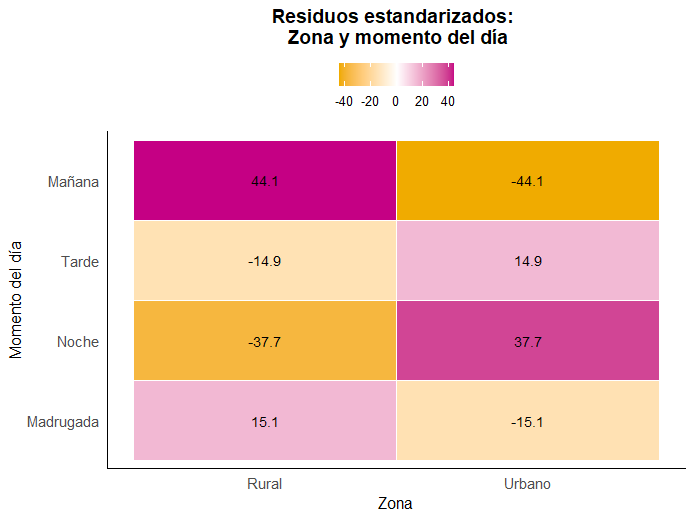
\includegraphics[width=0.5\textwidth]{Figuras/Residuos_horaZona.png}
        \caption{Residuos de zona (urbana o rural) y momento del día}
        \label{fig:residuo zona hora}
    \end{figure}

  Se sugiere que en las comunidades rurales las actividades productivas, agrícolas 
  y de desplazamiento hacia centros urbanos inician a horas muy tempranas, enfrentando 
  neblina, luz solar muy fuerte y carreteras resbaladizas por la lluvia matutina. 
  Por el contrario, el entorno urbano experimenta su mayor saturación de riesgo por 
  la noche debido al tráfico de ocio, las jornadas laborales y la reducción de visibilidad 
  en intersecciones complejas. Este comportamiento valida la visión de \textcite{HOSSEINIAN2012} 
  al demostrar que los picos de siniestralidad se alinean con las imperfecciones 
  de las rutinas sociales. El vacío de este modelo se ve en que la segmentación 
  en grandes bloques horarios impide capturar las fluctuaciones asociadas a las 
  "horas pico" de congestión vehicular extrema.
  
  A través de los resultados de las metodologías expuestas se encuentra que el 
  riesgo en las carreteras no se distribuye de manera uniforme ni es de forma 
  lineal a factores aislados, sino que sucede a partir de configuraciones espacio-temporales
  y de infraestructura del entorno vial en el que se esté. El primer resultado analiza 
  la interacción entre la condición de la superficie de la vía y la condición de la 
  luz, note \ref{tab:resumen_chicuadrado}. Al aplicar la prueba de independencia 
  Chi-cuadrado a estas variables categóricas, se obtuvo un valor p de $2,2 \times 10^{-16}$, 
  lo cual determina que existe una dependencia entre la superficie vial y las condiciones 
  de luz en la ocurrencia de accidentes. Además, el coeficiente V de Crámer da un valor 
  de $0,1151$, indicando que si bien la asociación es cierta en términos probabilísticos,
  su magnitud es débil debido a la magnitud de la cantidad de datos usados.

  Por otro lado, los resultados indican que la mayor cantidad de accidentes se concentra 
  de manera diurna sobre superficies secas. Esto se atribuye de forma lógica a 
  variables de exposición como la alta densidad del flujo vehicular y la congestión 
  en horas laborales, factores que multiplican exponencialmente las oportunidades 
  de colisión. No obstante, al aislar los residuos positivos significativos, se 
  descubren patrones locales importantes observados acontinuacion en \ref{fig:residuos superfice luz} 
  tales como que los accidentes sobre calles mojadas o inundadas se encuentran 
  fuertemente vinculados a los entornos de oscuridad con iluminación artificial 
  y a la oscuridad total, mientras que las calles con presencia de hielo o escarcha 
  muestran una asociación con la oscuridad en tramos sin alumbrado público.
    \begin{figure}[H]
        \centering
        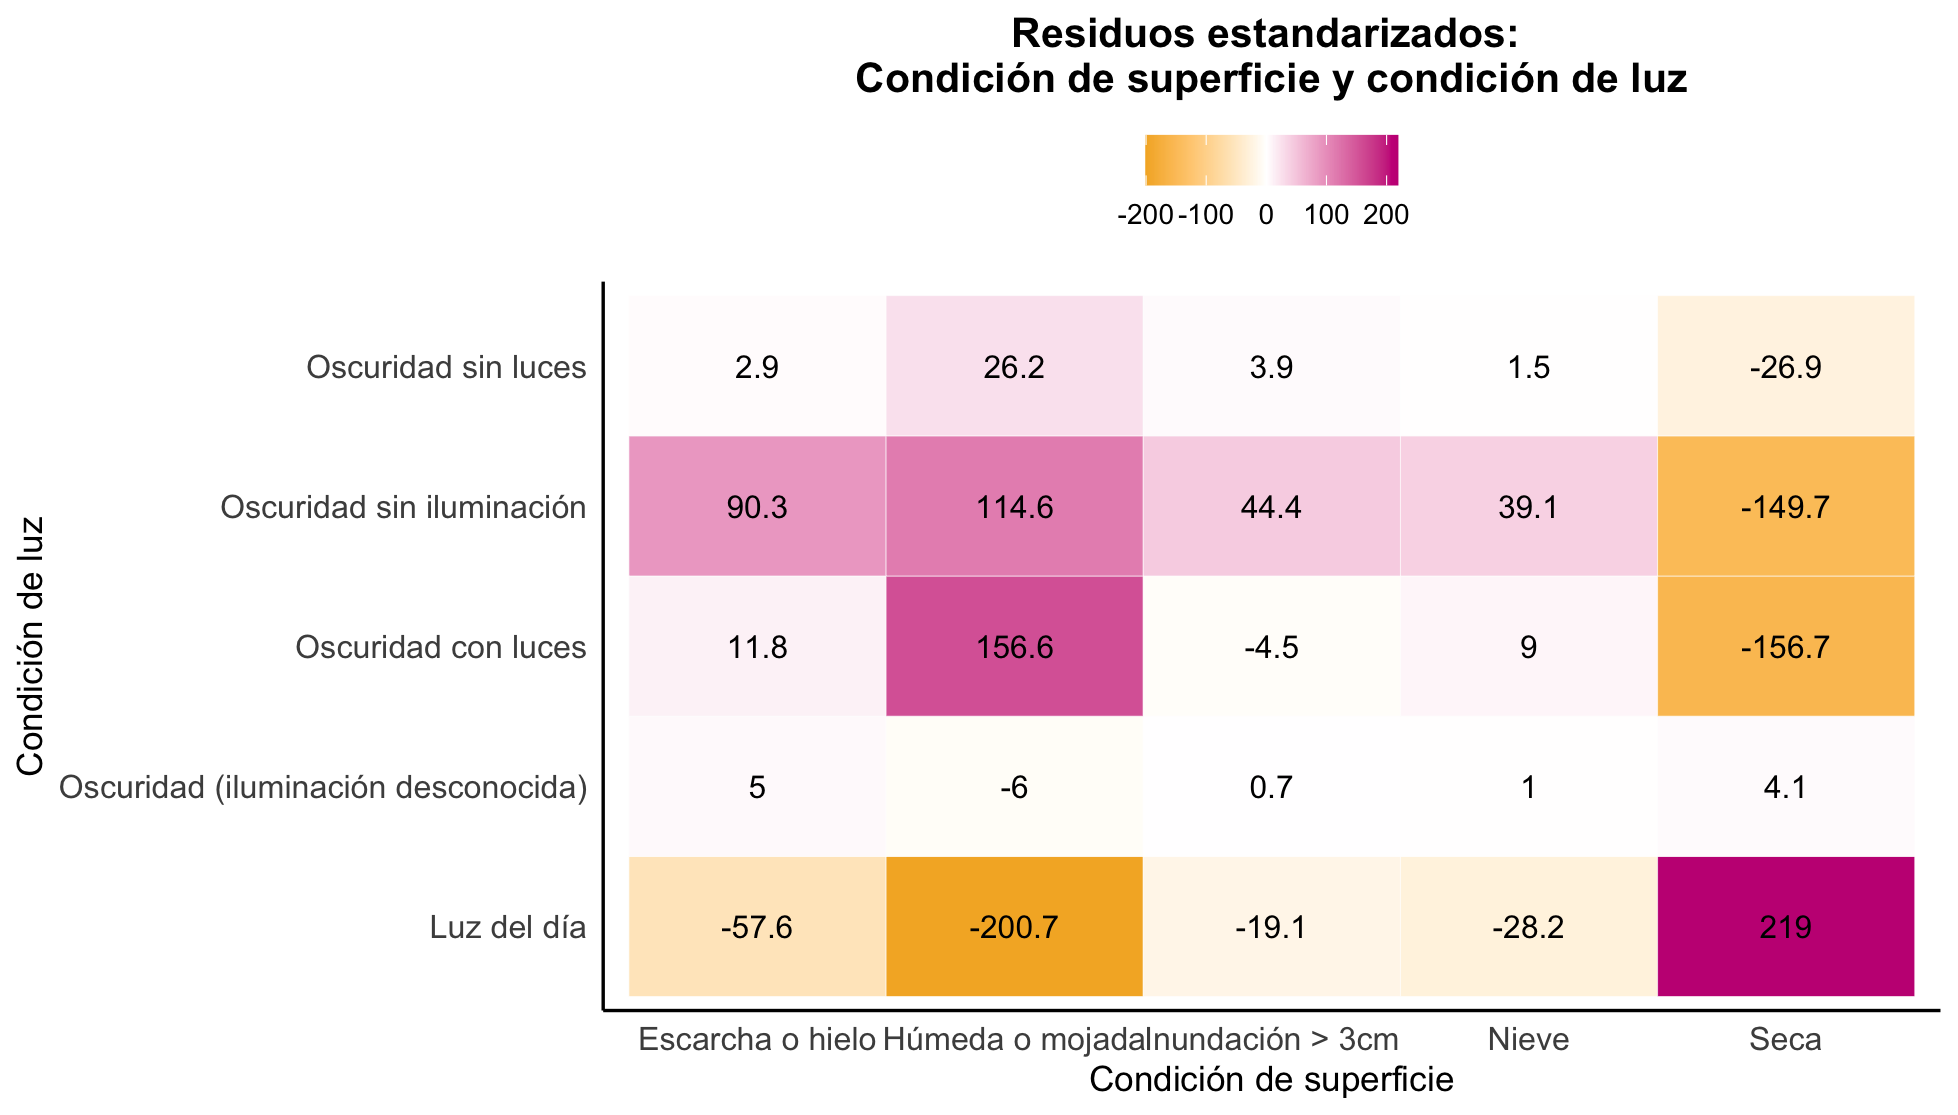
\includegraphics[width=0.6\textwidth]{Figuras/Residuos_superficie_luz.png}
        \caption{Residuos condición de superficie de la vía y condición luz}
        \label{fig:residuos superfice luz}
    \end{figure}

  Este comportamiento confirma lo que se menciona por \textcite{KARZAN2017} 
  en Greater Manchester, demostrando que la interacción entre la pérdida de 
  fricción neumática y la disminución de la agudeza visual del conductor 
  potencia la probabilidad de participar en un accidente. Sin embargo, no se puede 
  demostrar si el patrón diurno sobre superficie seca responde al peligro por el 
  diseño vial o simplemente a la concentración masiva de automóviles en circulación.

  Otro resultado es la evaluación entre las condiciones específicas de la superficie
  y el tipo de carretera, donde la prueba de Chi-cuadrado y el coeficiente V de
  Crámer mostradas en \ref{tab:resumen_chicuadrado} denotan que hay una dependencia, 
  pero al la V de Cramer estar cercana a 0 no es tan fuerte. Al evaluar los residuos 
  se encuentra que los factores que más riesgo implican son las carreteras que 
  presentan superficies alteradas por hielo, acumulación de nieve o inundaciones 
  localizadas. El hallazgo se relaciona con la investigación de \textcite{KARZAN2017}, 
  reforzando la idea de que los accidentes sobre carreteras donde los autos aumentan 
  su velocidad y sin detenerse, ocurren cuando la carretera se vuelve resbaladiza.

  Se analizó el vínculo entre las condiciones climáticas y la presencia de obstáculos 
  físicos, donde la prueba de Chi-cuadrado y la V de Crámer denotan que hay una 
  dependencia, pero débil. Los residuos graficados en \ref{fig:residuos_superficie_tipo_via} 
  logran identificar que hay un factor de riesgo cuando hay clima lluvioso y existen sustancias 
  deslizantes o defectos estructurales en la carretera. Este hallazgo se relaciona con 
  el trabajo de \textcite{KARZAN2017} con el papel del agua sobre las deficiencias 
  físicas del entorno vial, donde la precipitación no solo reduce la visibilidad de 
  los defectos en la carretera, sino que estas sustancias deslizantes anulan el buen
  funcionamiento del freno del automóvil provocando pérdidas de control.

    \begin{figure}[H]
        \centering
        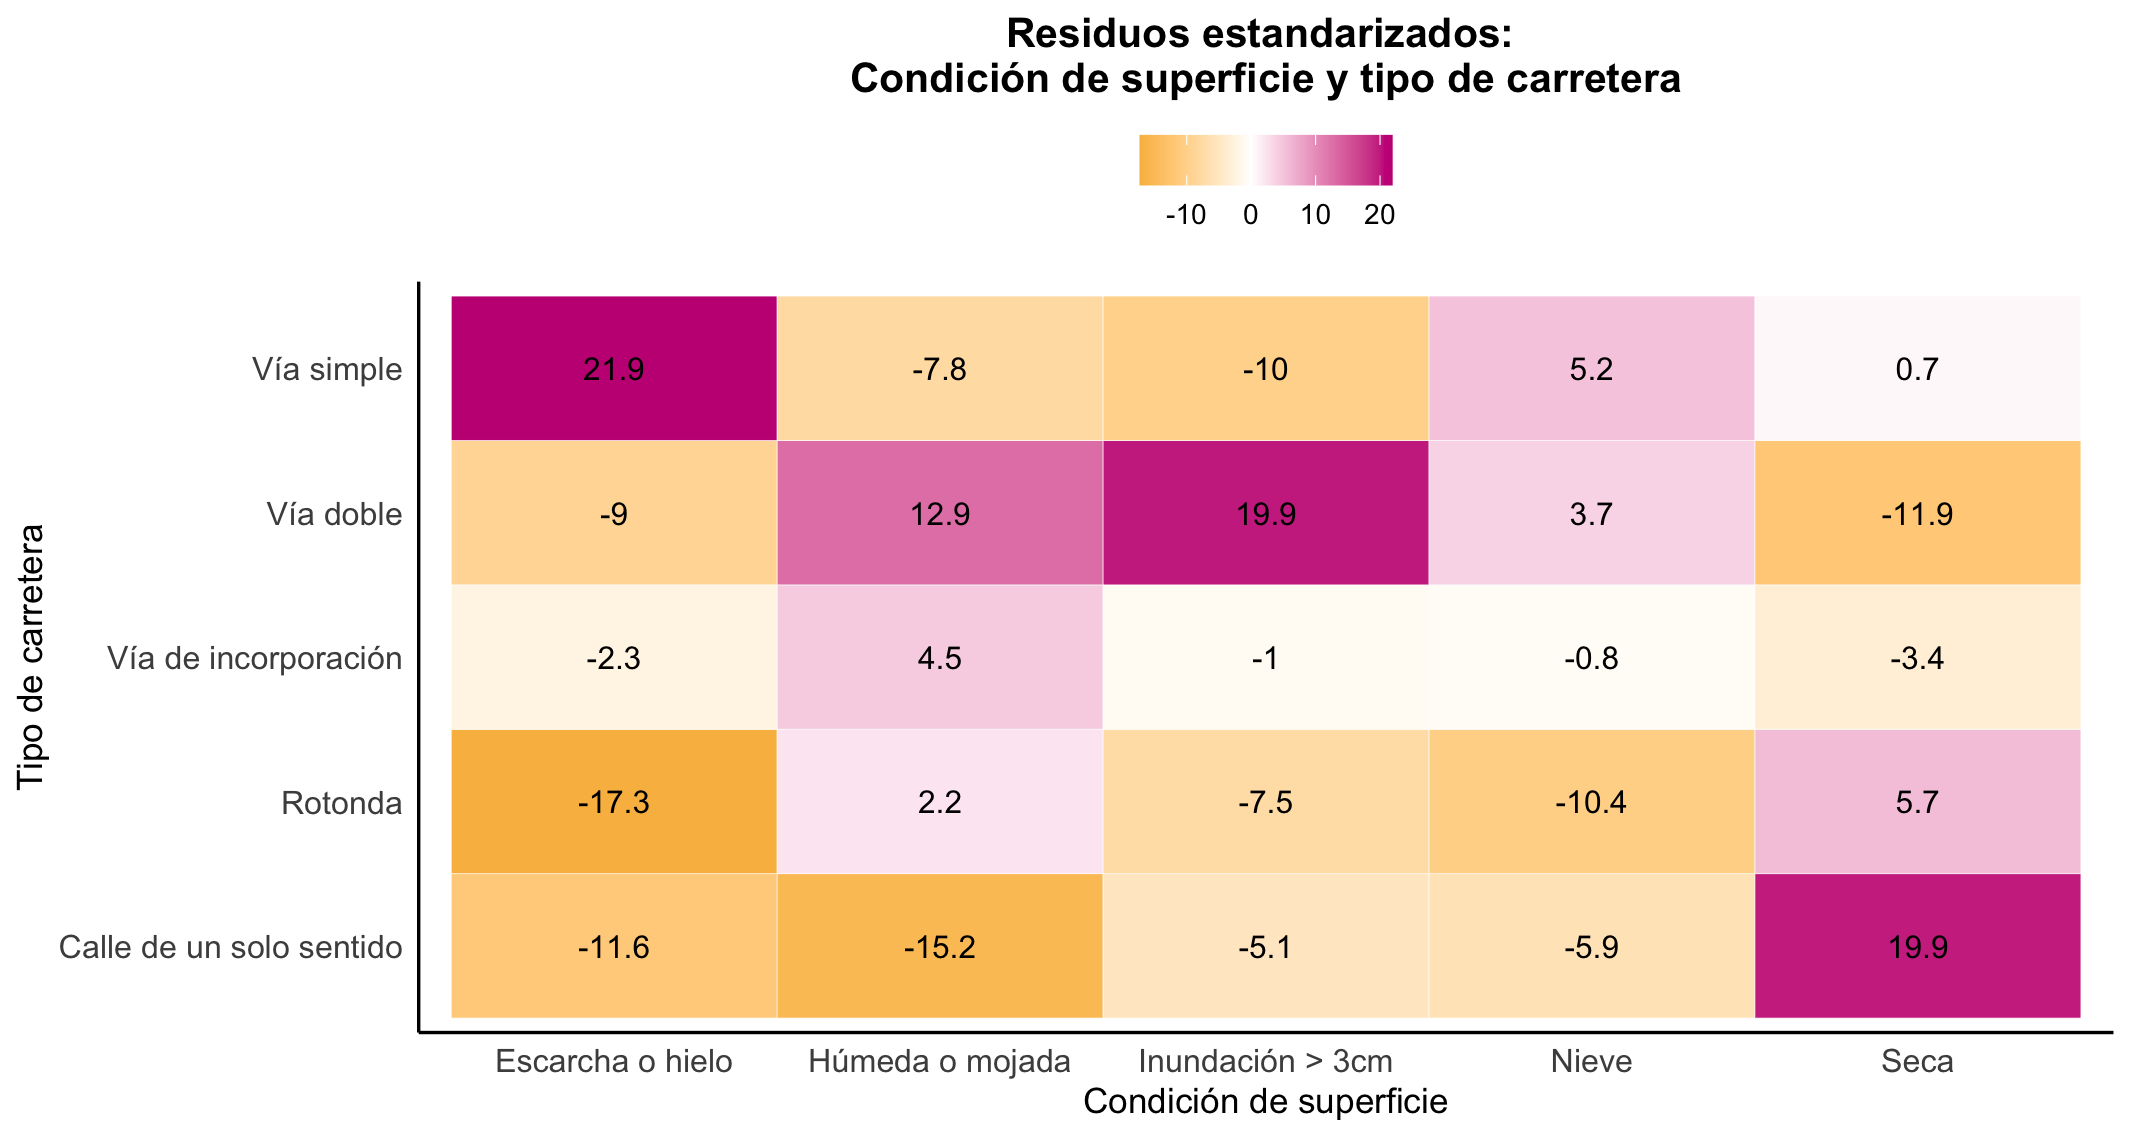
\includegraphics[width=0.6\textwidth]{Figuras/Residuos_superficie_tipodevia.png}
        \caption{Residuos de condición de superficie y tipo de vía}
        \label{fig:residuos_superficie_tipo_via}
    \end{figure}
  
  El análisis de la interacción entre iluminación y tipo de carretera mediante la 
  prueba Chi-cuadrado reveló una dependencia significativa observe la tabla \ref{tab:resumen_chicuadrado} 
  ($p\text{-valor} = 2,2 \times 10^{-16}$, V de Crámer $= 0,004974$), demostrando 
  mediante los residuos estandarizados que las carreteras de vías dobles en oscuridad 
  total registran accidentes muy superiores a los esperados, mostrado en \ref{fig:residuo iluminacion via}.
  Este riesgo se vincula a los principios de velocidad de \textcite{TAYLOR2000}, 
  ya que en estas vías de alta velocidad la falta de alumbrado público hace que 
  el espacio requerido para detener el vehículo exceda el límite visible iluminado
  por los faros, reduciendo el tiempo de reacción y por ende dificultando la 
  regulación de la velocidad en tiempo real ante imprevistos.

    \begin{figure}[H]
        \centering
        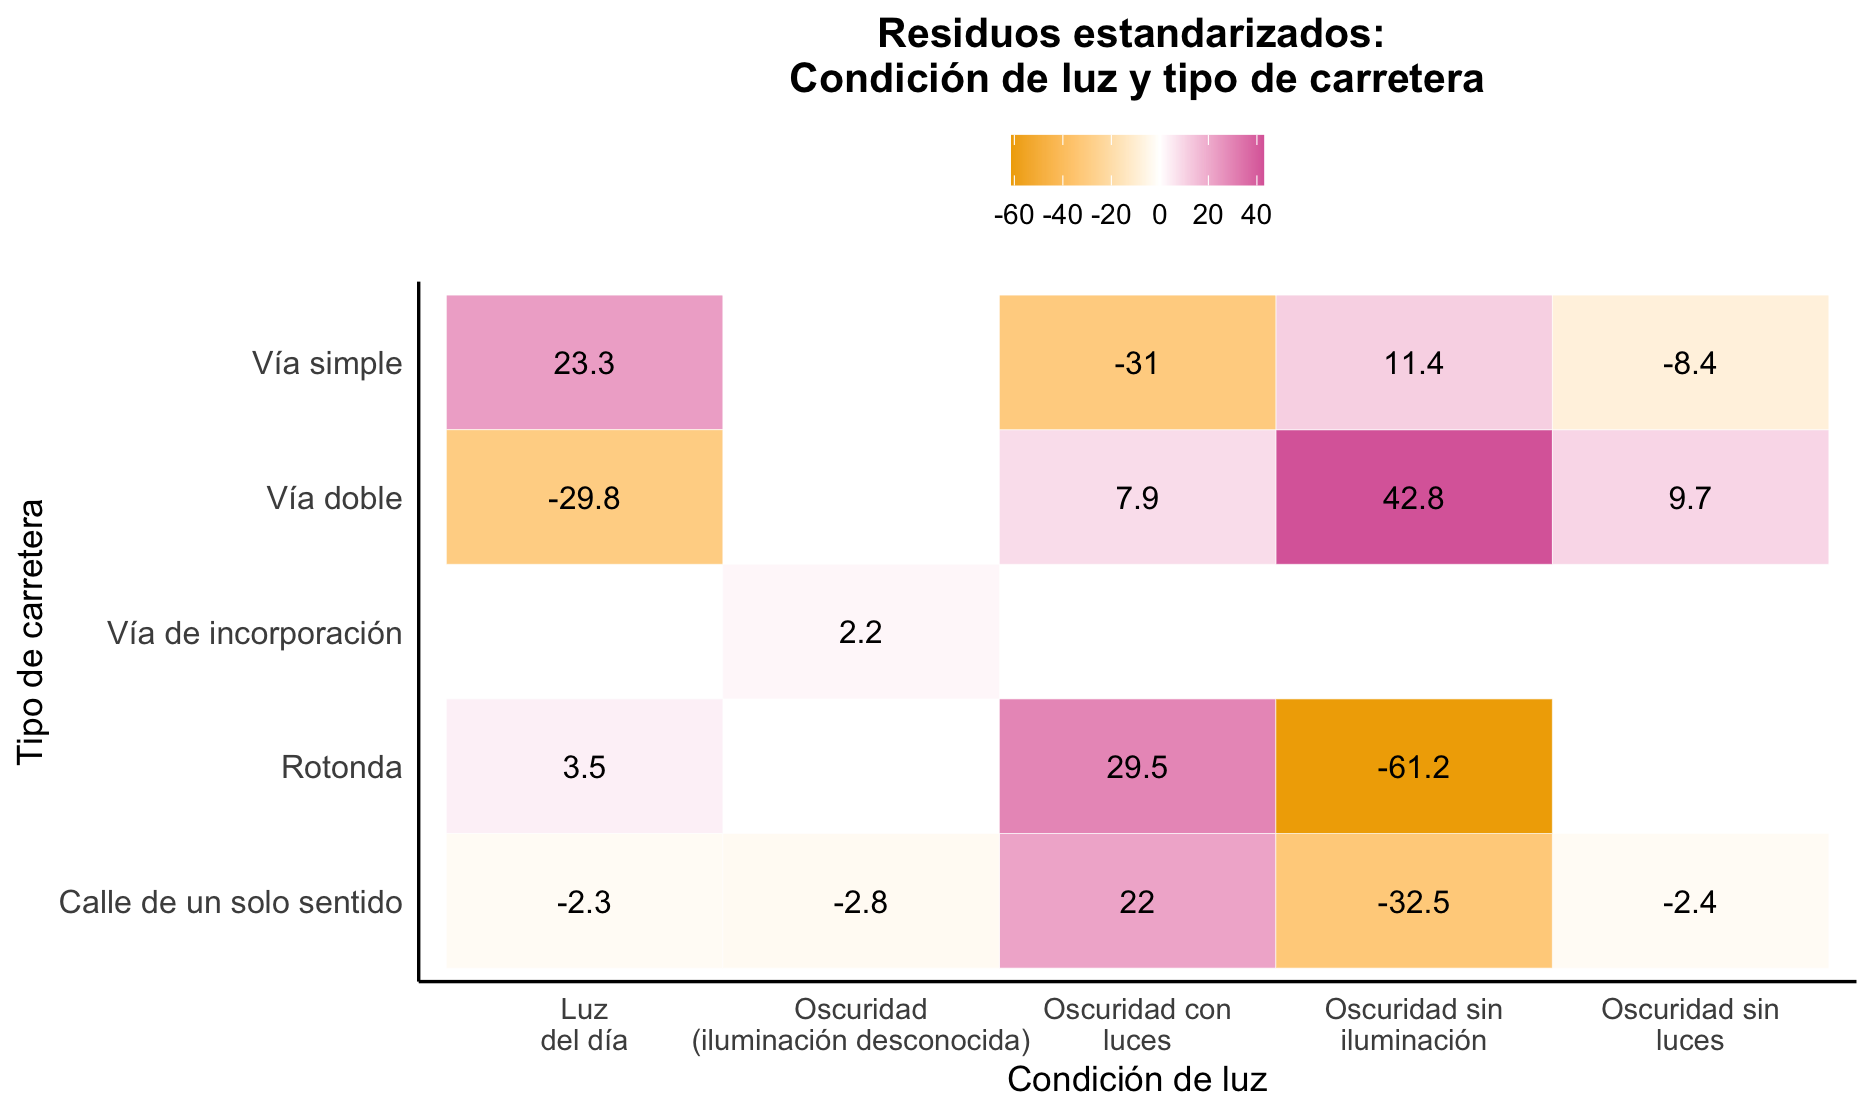
\includegraphics[width=0.6\textwidth]{Figuras/Residuos_ilum_via.png}
        \caption{Residuos de condición de luz y tipo de vía}
        \label{fig:residuo iluminacion via}
    \end{figure}

    
    
\textbf{Conclusiones:}
  El presente estudio identificó combinaciones de factores del entorno más frecuentes en los accidentes de tránsito del Reino Unido (2010-2017). Se adoptó este enfoque para entender la interacción de los factores y mitigar la siniestralidad. Inicialmente se esperaba un riesgo concentrado en condiciones adversas, sin embargo, los resultados mostraron más colisiones en condiciones óptimas debido a la alta exposición vehicular. No obstante, al aislar los residuos estadísticos, los hallazgos coincidieron con la teoría: se evidenciaron patrones en la interacción de altas velocidades con superficies mojadas/hielo, y oscuridad total en vías dobles.
  La metodología de Chi-cuadrado y la V de Crámer resolvió la pregunta aislando asociaciones mediante residuos estandarizados. Como problemas, la exclusión de valores faltantes obligó a indexarlos para no perder información esencial. Además, la muestra masiva provocó que los p-valores fueran altamente significativos ($p < 2,2 \times 10^{-16}$) pero con magnitudes de V de Crámer débiles ($0,004$ a $0,115$), limitando la prueba al detectar dependencias reales pero con una fuerza de asociación disminuida por el volumen de datos. Para futuros trabajos, se recomienda utilizar modelos multivariados avanzados que midan el impacto simultáneo y controlado de varios factores.
  Este trabajo resuelve un vacío en la literatura al expandir el análisis a escala nacional durante ocho años, superando el enfoque aislado de estudios previos en entornos locales o curvas. Al validar la Teoría del Dominó y el Modelo de Múltiples Causas, demuestra que las anomalías del entorno actúan como fichas imprevistas que rompen la homeostasis del riesgo del conductor, aportando información clave para políticas públicas de seguridad vial.\\

  \textbf{Agradecimientos:}
Nos gustaría expresar nuestro más sincero agradecimiento al Dr. Maikol Solis por 
su orientación, apoyo y acompañamiento durante el desarrollo de esta investigación. 
Sus conocimientos, observaciones y recomendaciones fueron fundamentales para la 
correcta aplicación de las metodologías planteadas y fortalecer el análisis realizado. 
\newpage
\printbibliography

\subsection{Anexos:}

\textbf{Resumen de pruebas Chi-cuadrado de independencia y V de Crámer}
\begin{table}[htbp]
\centering
\resizebox{0.85\textwidth}{!}{
\begin{tabular}{p{11.5cm}cc}
\toprule
\textbf{Variables cruzadas} & \textbf{\textit{p}-valor} & \textbf{V de Crámer} \\
\midrule

Condición de superficie $\times$ Condición de luz &
$< 2.2 \times 10^{-16}$ & 0.1151 \\

Condición de superficie $\times$ Límite de velocidad &
$< 2.2 \times 10^{-16}$ & 0.0974 \\

Zona $\times$ Momento del día &
$< 2.2 \times 10^{-16}$ & 0.0497 \\

Detalles de intersección $\times$ Condiciones especiales de la carretera &
$< 2.2 \times 10^{-16}$ & 0.0449 \\

Día de la semana $\times$ Zona &
$< 2.2 \times 10^{-16}$ & 0.0432 \\

Condición de luz $\times$ Tipo de carretera &
$< 2.2 \times 10^{-16}$ & 0.0405 \\

Condición climática $\times$ Condiciones especiales de la carretera &
$< 2.2 \times 10^{-16}$ & 0.0261 \\

Condición de superficie $\times$ Tipo de carretera &
$< 2.2 \times 10^{-16}$ & 0.0191 \\

\bottomrule
\end{tabular}
}
\footnotesize
\caption{Resumen de las pruebas Chi-cuadrado de independencia y fuerza de asociación (V de Crámer)}
\label{tab:resumen_chicuadrado}
\end{table}

\end{document}

